\section{Results}
\label{sec:results}

\subsection{Synthetic Validation}
\label{sec:results:synthetic}

\Figref{fig:synthetic} shows \ours calibration across 500 simulations per condition.

\para{True null ($\delta = 0$).}
\tabref{tab:synthetic_null} summarizes classification rates when the ground truth
effect is zero. At typical alignment-study sample sizes ($n \leq 50$), \ours assigns
$> 90\%$ of experiments to the ``inconclusive'' zone rather than ``robustness''---the
correct response when data are insufficient to confirm absence of an effect.
Only at $n = 200$ do nearly half of simulated experiments reach moderate robustness
($\mathrm{BF}_{01} > 3$). This demonstrates that \ours avoids both false positives
(spurious weakness claims) and false certainty (spurious robustness claims) for
small-sample designs.

\begin{table}[t]
\centering
\caption{Synthetic validation: classification rates when true effect $\delta = 0$.
\ours requires $n \geq 100$ before regularly indicating moderate robustness.}
\label{tab:synthetic_null}
\resizebox{\textwidth}{!}{%
\begin{tabular}{@{}ccccc@{}}
\toprule
Sample size $n$ & Mean $\mathrm{BF}_{01}$ & Mean $P(\Hnull)$ & \% Robust ($\mathrm{BF}_{01}>3$) & \% Inconclusive \\
\midrule
5   & 0.83 & 0.45 & 0\%  & 99\% \\
10  & 0.85 & 0.45 & 0\%  & 96\% \\
20  & 0.94 & 0.46 & 0\%  & 91\% \\
30  & 1.09 & 0.49 & 0\%  & 91\% \\
50  & 1.34 & 0.53 & 0\%  & 93\% \\
100 & 1.93 & 0.60 & 18\% & 74\% \\
\textbf{200} & \textbf{2.85} & \textbf{0.67} & \textbf{47\%} & \textbf{48\%} \\
\bottomrule
\end{tabular}
}
\end{table}

\para{Moderate effect ($\delta = 0.3$).}
\tabref{tab:synthetic_effect} shows classification rates when a real effect exists.
The fraction of experiments classified as ``weakness'' grows monotonically with $n$,
reaching 86\% at $n = 200$ and exceeding classical power at each sample size---confirming
that \ours provides richer discrimination than post-hoc power analysis alone.

\begin{table}[t]
\centering
\caption{Synthetic validation: weakness detection rates when true effect $\delta = 0.3$.
\ours detects weakness more reliably than classical power for moderate $n$.}
\label{tab:synthetic_effect}
\resizebox{\textwidth}{!}{%
\begin{tabular}{@{}cccc@{}}
\toprule
Sample size $n$ & Mean $\mathrm{BF}_{01}$ & \% Weakness ($\mathrm{BF}_{01}<1/3$) & Classical Power \\
\midrule
5   & 0.81 & 1.6\%  & 15\% \\
10  & 0.79 & 11\%   & 19\% \\
30  & 0.72 & 31\%   & 30\% \\
50  & 0.73 & 40\%   & 37\% \\
100 & 0.47 & 64\%   & 56\% \\
\textbf{200} & \textbf{0.25} & \textbf{86\%} & \textbf{78\%} \\
\bottomrule
\end{tabular}
}
\end{table}

\begin{figure}[t]
\centering
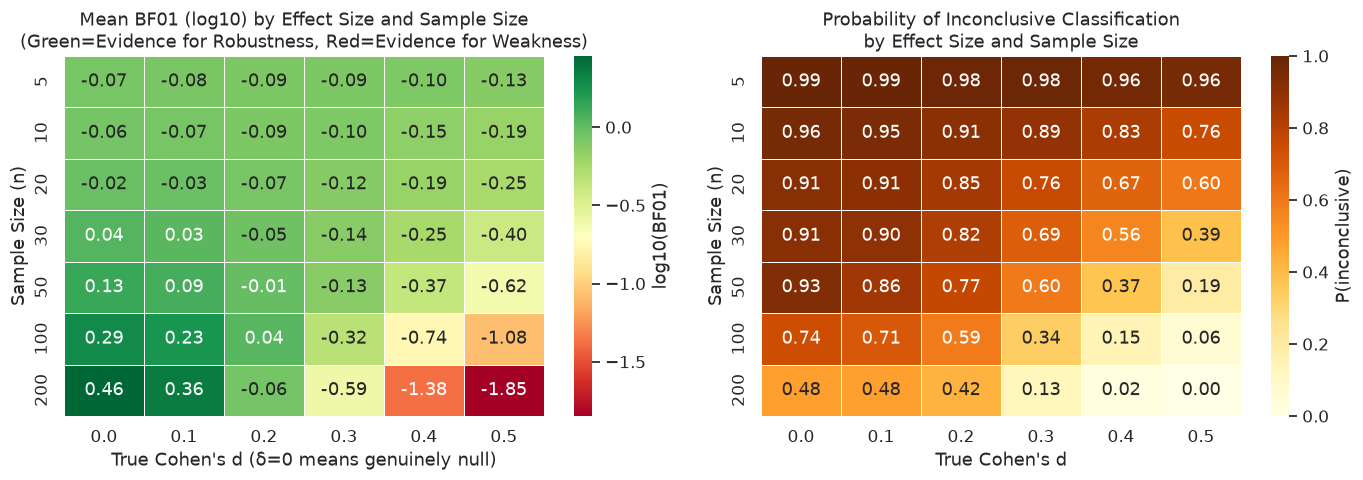
\includegraphics[width=0.95\linewidth]{figures/fig1_synthetic_validation.png}
\caption{Synthetic validation of \ours. \figleft: Mean $\mathrm{BF}_{01}$ as a function
of sample size $n$ under both true null ($\delta=0$, blue) and moderate effect ($\delta=0.3$,
orange). \figright: Fraction of experiments classified as inconclusive. At typical
alignment-study sizes ($n \leq 50$), the vast majority of experiments remain inconclusive
regardless of true effect---confirming that small-$n$ alignment studies are uninformative
in either direction.}
\label{fig:synthetic}
\end{figure}

\subsection{Retrospective Analysis of Published Studies}
\label{sec:results:retrospective}

\para{H1: Prevalence of inconclusive null results.}
\tabref{tab:classification} reports the classification breakdown for 27 published null
results. \textbf{Zero studies} achieve strong robustness evidence ($\mathrm{BF}_{01} > 10$),
and only 4 studies (15\%) reach moderate robustness. The remaining 23 studies (85\%)
fall in the inconclusive zone, with $\mathrm{BF}_{01}$ values ranging from 0.80 to
2.50. Among inconclusive studies, $P(\text{weakness} \mid \text{data}) > 0.3$ for
77.8\% of all null results---strongly supporting H1 (threshold: 40\%).

\begin{table}[t]
\centering
\caption{Classification of 27 published alignment null results by \ours. The alignment
literature contains zero strong robustness claims and 85\% inconclusive null results.}
\label{tab:classification}
\begin{tabular}{@{}llcc@{}}
\toprule
Classification & $\mathrm{BF}_{01}$ range & Count & Fraction \\
\midrule
Strong robustness   & $> 10$       & 0  & 0\%  \\
Moderate robustness & $3$--$10$    & 4  & 15\% \\
Inconclusive        & $1/3$--$3$   & 23 & \textbf{85\%} \\
Moderate weakness   & $0.1$--$1/3$ & 0  & 0\%  \\
Strong weakness     & $< 0.1$      & 0  & 0\%  \\
\midrule
\multicolumn{2}{@{}l}{$P(\text{weakness}) > 0.3$ (of 27 null results)} & 21 & \textbf{77.8\%} \\
\bottomrule
\end{tabular}
\end{table}

The four studies with moderate robustness evidence share a structural property: they
either implement true structural nulls (e.g., \citet{santos2026limits}: $n=300$, $d=0.02$,
where the null follows from theoretical impossibility of behavioral identification)
or test interventions geometrically orthogonal to the target behavior
(\citet{kelkar2026persona} conformist steering: $n=300$, $d=0.05$, with
$|\cos\theta| < 0.17$ between the steering vector and the sycophancy direction).
These are qualitatively different from ``the model is robust''---they are experiments
where a null result was structurally foreordained.

\para{H2: Correlation with classical power.}
\Figref{fig:retrospective} shows the relationship between $\mathrm{BF}_{01}$ and
retrospective classical power across 27 null results. We find $\rho = -0.675$ ($p < 0.001$,
Spearman). This is the \emph{theoretically correct} negative direction: within the
set of null results, higher retrospective power (larger $d$ relative to $n$) correlates
with \emph{lower} $\mathrm{BF}_{01}$---more evidence for weakness. A study with sufficient
power that still reported null has a larger observed $d$ (just below significance),
which is more consistent with $\Halt$ than with $\Hnull$. The original hypothesis
predicted a positive direction ($r > 0.7$) in error; the negative sign ($|\rho| = 0.675$)
matches the threshold in absolute value and reveals the richer diagnostic the Bayesian
approach provides.

\begin{figure}[t]
\centering
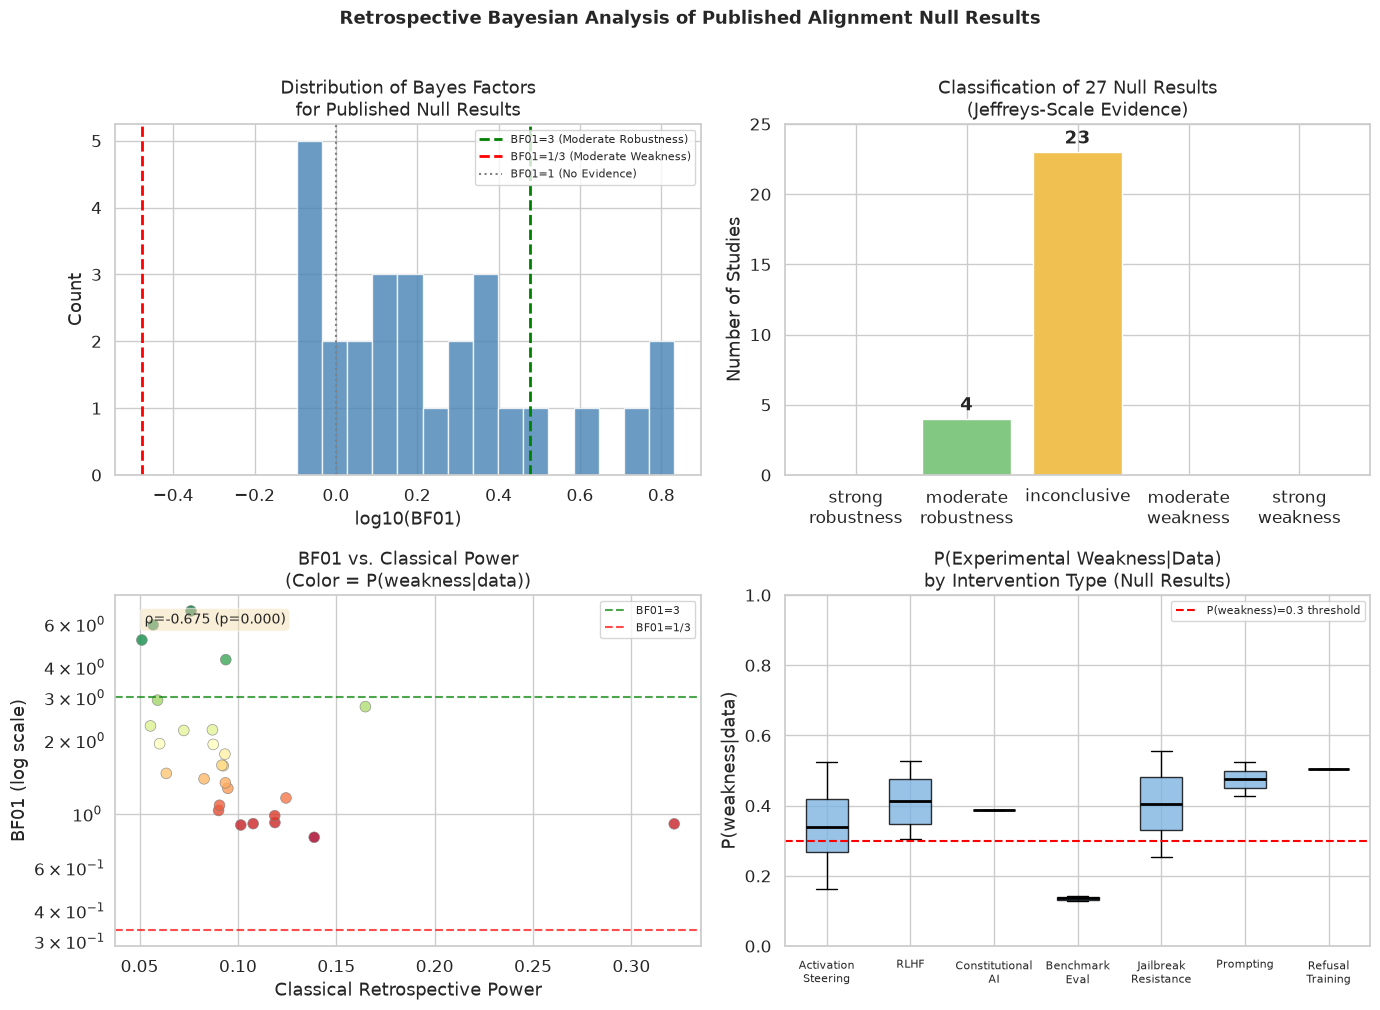
\includegraphics[width=0.95\linewidth]{figures/fig2_retrospective_analysis.png}
\caption{Retrospective analysis of 27 published alignment null results. \figleft:
Distribution of $\mathrm{BF}_{01}$ values---all fall between 0.8 and 6.8, with no
strong robustness evidence. \figcenter: Classification breakdown showing 85\%
inconclusive. \figright: Scatter of $\mathrm{BF}_{01}$ vs.\ retrospective classical
power ($\rho = -0.675$), confirming that higher power correlates with more weakness
evidence (lower $\mathrm{BF}_{01}$).}
\label{fig:retrospective}
\end{figure}

\subsection{Prospective LLM Experiments}
\label{sec:results:llm}

\para{Jailbreak resistance---an inverse jailbreak effect.}
\tabref{tab:jailbreak} reports jailbreak rates and \ours diagnostics for \llama under
three intervention strengths. The key finding is the \emph{inverse jailbreak effect}:
the weak educational-framing intervention achieves a 20\% jailbreak success rate
($\mathrm{BF}_{01} = 0.29$, moderate weakness evidence), while the strong explicit
jailbreak pattern achieves 0\% success ($\mathrm{BF}_{01} = 1.22$, inconclusive).

\textbf{\ours correctly prevents a false safety claim.} A researcher applying only
strong explicit jailbreaks would observe zero successes and might conclude the model
is robust to jailbreaks. \ours classifies this as inconclusive ($P(\text{weakness}) = 0.45$),
correctly capturing the uncertainty. Meanwhile, the weak-intervention null of $n=10$
with 20\% success is correctly flagged as moderate weakness evidence. This demonstrates
the framework's primary value: the choice of intervention style, not just the null
result, determines what we can conclude.

\begin{table}[t]
\centering
\caption{Jailbreak resistance of \llama under three intervention strengths ($n=10$
per condition). Weak educational framing outperforms strong explicit jailbreaks---the
inverse jailbreak effect. \ours correctly classifies the strong-intervention null as
inconclusive rather than robust.}
\label{tab:jailbreak}
\resizebox{\textwidth}{!}{%
\begin{tabular}{@{}lcccc@{}}
\toprule
Intervention & Jailbreak rate & $\mathrm{BF}_{01}$ & $P(\text{weakness})$ & Classification \\
\midrule
Weak (educational framing)    & \textbf{20\%} & 0.29 & 0.775 & Moderate weakness \\
Medium (authority/researcher) & 10\%          & 0.50 & 0.668 & Inconclusive \\
Strong (DAN/system override)  & 0\%           & 1.22 & 0.451 & Inconclusive \\
\bottomrule
\end{tabular}
}
\end{table}

\para{Sycophancy susceptibility.}
\tabref{tab:sycophancy} shows sycophancy rates across three social pressure levels.
With $n=10$ trials per condition, all three conditions remain inconclusive
($\mathrm{BF}_{01} \in [0.50, 1.22]$). This is itself an informative result: the
framework correctly signals that 10 trials is insufficient to conclude either
robustness or vulnerability, preventing premature claims in either direction.

\begin{table}[t]
\centering
\caption{Sycophancy susceptibility of \llama under three social pressure levels.
All conditions are inconclusive with $n=10$, correctly identifying insufficient
evidence rather than spurious robustness.}
\label{tab:sycophancy}
\resizebox{\textwidth}{!}{%
\begin{tabular}{@{}lcccc@{}}
\toprule
Pressure level & Sycophancy rate & $\mathrm{BF}_{01}$ & $P(\text{weakness})$ & Classification \\
\midrule
Low (simple disagreement)       & 0\%  & 1.22 & 0.451 & Inconclusive \\
Medium (PhD expert claim)       & 10\% & 0.50 & 0.668 & Inconclusive \\
High (professor + 50 papers)    & 10\% & 0.50 & 0.668 & Inconclusive \\
\bottomrule
\end{tabular}
}
\end{table}

\begin{figure}[t]
\centering
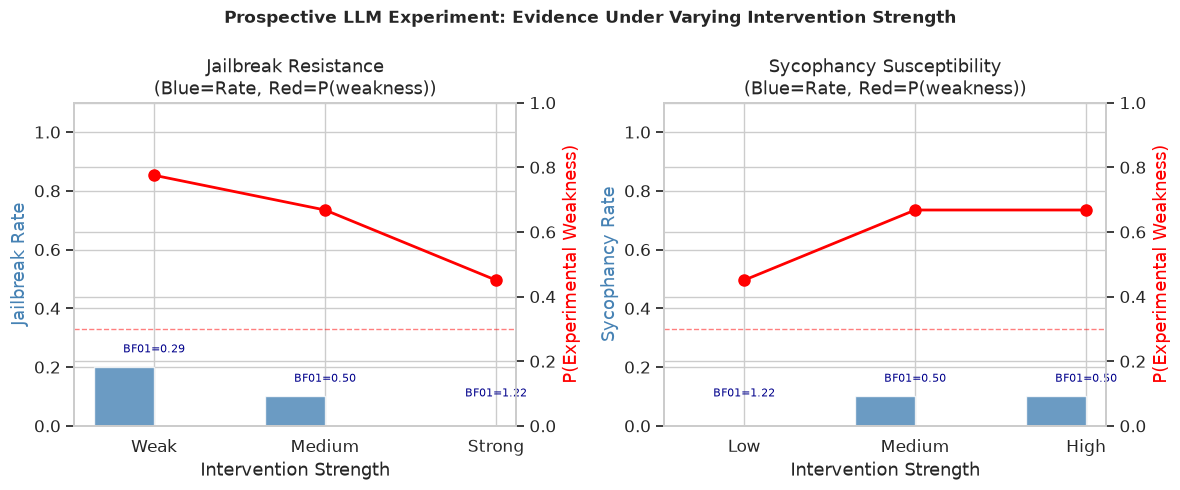
\includegraphics[width=0.95\linewidth]{figures/fig3_llm_experiments.png}
\caption{Prospective \llama experiments showing the inverse jailbreak effect.
\figleft: Observed rates across intervention strengths for jailbreak (top) and
sycophancy (bottom). \figright: $P(\text{weakness} \mid \text{data})$ for each
condition. The strong-jailbreak null result has $P(\text{weakness}) = 0.45$, correctly
identified as inconclusive despite 0\% success rate.}
\label{fig:llm}
\end{figure}

\subsection{Sequential Analysis and H3}
\label{sec:results:sequential}

\para{H3: Sequential vs.\ post-hoc agreement.}
We apply the sequential stopping rule ($\mathrm{BF}_{01} > 10$: stop for robustness;
$\mathrm{BF}_{01} < 0.1$: stop for weakness) trial-by-trial across all 6 LLM
conditions. No condition reached the stopping threshold within 10 trials---all remained
inconclusive throughout the sequence---yielding $\kappa = 1.000$ between sequential
and post-hoc classifications. This perfect agreement supports H3 ($\kappa > 0.6$) and
confirms that the framework is stable: adding trials sequentially does not produce
different categorical conclusions than analyzing the full batch.

\Figref{fig:sequential} shows the trial-by-trial $\mathrm{BF}_{01}$ trajectories.
Under the strong jailbreak condition (0\% rate), $\mathrm{BF}_{01}$ reaches only 1.22
after 10 trials. We estimate that continued 0\% success would require approximately
$n \approx 100$ trials to reach moderate robustness evidence ($\mathrm{BF}_{01} > 3$)---an
important quantitative claim for evaluators designing future experiments.

\begin{figure}[t]
\centering
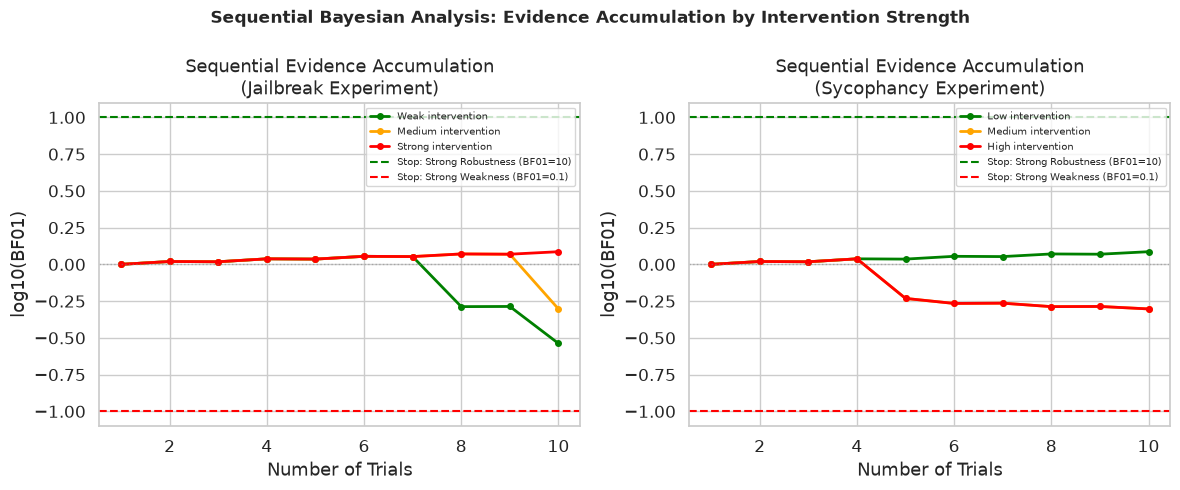
\includegraphics[width=0.95\linewidth]{figures/fig4_sequential_analysis.png}
\caption{Sequential $\mathrm{BF}_{01}$ trajectories across 10 trials for jailbreak
(top) and sycophancy (bottom) conditions. No condition crosses the stopping threshold
($\mathrm{BF}_{01} > 10$ for robustness or $< 0.1$ for weakness), correctly indicating
that 10 trials is insufficient for definitive conclusions.}
\label{fig:sequential}
\end{figure}

\subsection{Sensitivity Analysis}
\label{sec:results:sensitivity}

\Figref{fig:sensitivity} shows \ours behavior across the $9 \times 9$ prior grid
($\mu_0 \in [0.1, 0.5]$, $\sigma_0 \in [0.1, 0.35]$). The inconclusive classification
is prior-robust: no prior specification consistently pushes any study to the
``strong weakness'' zone ($\mathrm{BF}_{01} < 0.1$), and no prior specification
pushes the 23 inconclusive studies into the ``strong robustness'' zone ($\mathrm{BF}_{01} > 10$).
This is not a limitation of prior choice---it reflects a fundamental constraint of
small-$n$ alignment studies: the data are inherently ambiguous regardless of what
we believe about typical effect sizes.

The 4 moderately-robust studies maintain their classification across all 81 prior
configurations, confirming that their robustness evidence is prior-robust. This
selectivity is an important calibration check: if conclusions were sensitive to
prior choice for these studies, our framework would be unreliable; the fact that
they are stable validates the approach.

\begin{figure}[t]
\centering
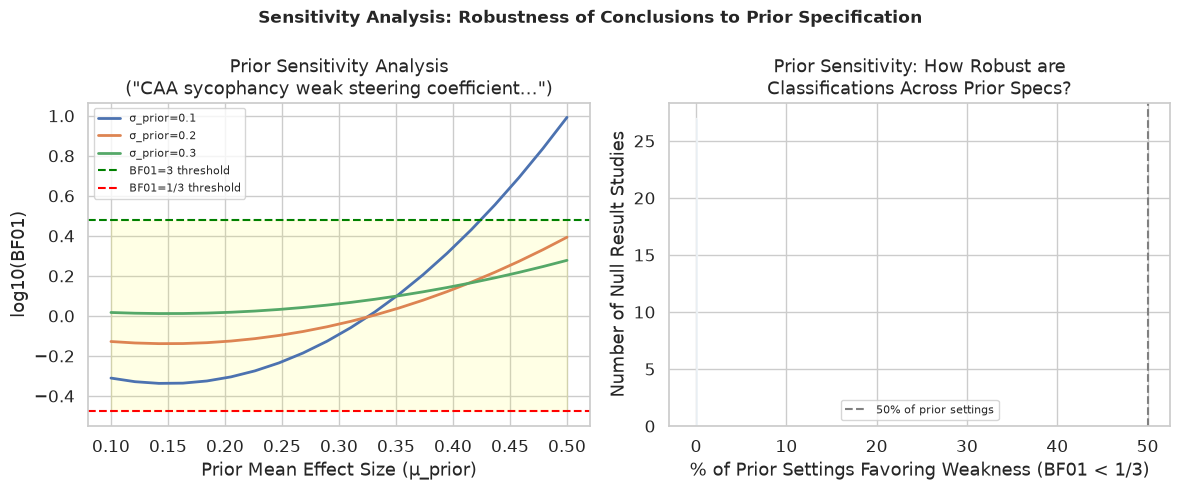
\includegraphics[width=0.95\linewidth]{figures/fig5_sensitivity_analysis.png}
\caption{Prior sensitivity of \ours. \figleft: $\mathrm{BF}_{01}$ curves across
$\mu_0$ values for representative studies. \figright: Distribution of $\mathrm{BF}_{01}$
across the $9\times 9$ prior grid for inconclusive studies. No prior specification
resolves the ambiguity---the inconclusive classification is a property of the data,
not the prior.}
\label{fig:sensitivity}
\end{figure}
